% kapitel2.tex
\chapter{Grundlagen}
\label{chapter:grundlagen}
\section{Smart Home}
Im Zuge der Digitalisierung und Vereinfachung der Beschaffung von Sensorik im Alltag ist Smart Home als Konzept für den Verbraucher angekommen und bezahlbar. Dabei handelt es sich im allgemeinsten Fall um eine Basisstation mit beliebig vielen Akteuren und Sensoren. Jene Station dient dem verarbeiten und speichern der Daten aus den sensorischen Elementen des Verbundes und anhand von zum Beispiel Entscheidungstabellen werden dann die Akteure angesteuert. Als simples Szenario kann man sich hier eine Wohnzimmerlampe vorstellen, welche angeschaltet wird, wenn der draußen angebrachte Helligkeitssensor Dunkelheit signalisiert. Allerdings muss ein System nicht zwangsläufig Sensoren und Akteure haben. Ein Netzwerk aus Sensoren würde nur überwachen und eines aus Akteuren kann nur handeln. Beispiele hierfür wären eine zentrale Stromverbrauchüberwachung pro Steckdose oder eine Heizungssteuerung.
Hierbei gibt es noch zu erwähnen, dass es auch Kombigeräte gibt. Ein Heizungsthermostat hat meist ein eingebautes Thermometer und ist somit Akteur und Sensor.\\

\begin{figure}[!h]
	\centering
	\begin{tikzpicture}[every text node part/.style={align=center}]
	\node[] (A) {
\includegraphics[width=50px]{./assets/images/plug-solid}\\Sensor};
	\node[right= 3cm of A] (B) {
\includegraphics[width=50px]{./assets/images/chalkboard-solid}\\Basisstation};
	\node[right= 3cm of B] (C) {
\includegraphics[width=50px]{./assets/images/lightbulb-solid}\\Akteur};
	\draw[-{Stealth[scale=1.3,angle'=90]},semithick] (B) -- node[above] {0..N} (A) ;
	\draw[-{Stealth[scale=1.3,angle'=90]},semithick] (B) -- node[above] {0..M} (C) ;
	\end{tikzpicture}
\end{figure}
\section{Grundbegriffe}
Im Kontext von Prometheus und dieser Arbeit sind ein paar potentiell mehrdeutiger Begriffe genauer zu spezifizieren.
\subsection{Metriken}
Eine Eigenschaft welche beobachtet und gemessen wird.
\begin{Beispiel}
	Temperatur, Regenmenge, Helligkeit, Transferrate, gedruckte Dokumente
\end{Beispiel}
\begin{Definition}
	Eine Metrik ist eine einzige, zu messende Eigenschaft.
\end{Definition}
\subsection{Sensor}
Ein Sensor ist ein reelles Gerät, eine Einheit welche in der echten Welt eingesetzt wird. Dieses kann mehrere Metriken erfassen und sie dann über eine Schnittstelle zur Verfügung stellen.
\begin{Beispiel}
	Wetterstation, Netzwerkswitch, Heizungsthermostat
\end{Beispiel}
\begin{Definition}
	Eine Metrik ist eine einzige zu messende Eigenschaft.
\end{Definition}

\section{Prometheus}
Bei Prometheus handelt es sich um eine Open Source Lösung die zur Überwachung von Metriken und der Alarmierung dient. Es gibt die Möglichkeit Daten aktiv zu übergeben oder alternativ Prometheus so zu konfigurieren und damit zu beauftragen, dass es sich die Daten von verschiedenen Datenquellen abholt. Für die letztere Variante muss das zu Überwachende System eine HTTP Schnittstelle zur Verfügung stellen auf der in einer Vordefinierten Art die Daten ausgeliefert werden. Um diesen Prozess zu vereinfachen gibt es bereits verschiedene Libraries für verschiedene Programmiersprachen die konfigurativ ein solches Format einhalten. Zum Zeitpunkt des Schreibens sind offiziel GO, Scala/Java, Python und Ruby unterstützt, allerdings gibt es für zahlreiche andere Sprachen unoffizielle Third Party Libraries welche auf der Internetseite von Prometheus beworben werden. Für den Fall, dass die gewählte Sprache nicht unterstützt wird ist es auch möglich die Ausgabe selber zu erstellen. Dafür ist die Definition des Ausgabeformat gut dokumentiert worden. 
\subsection{Zählertypen}
Prometheus unterscheidet bei Metriken zwischen verschiedenen Typen. Nachfolgen werden alle Möglichkeiten kurz Erläutern. Im \autoref{subsec:Exportformat}  für das Verständnis ein paar Beispiele aufgelistet und erklärt.
\subsubsection{Counter}
Der Counter beschreibt eine Metrikart, welche nur hochgezählt und zurückgesetzt werden kann. Sie stellt eine monoton wachsende Funktion dar. 
\subsubsection{Gauge}
Dieser Typ symbolisiert eine Messuhr oder Tachometer. Die Werte können steigen und fallen.
\subsubsection{Histogram}
Bei einem Histogramm handelt es sich um ein Konzept bestehend aus sogenannten Buckets. Diese werden initial für eine Metrik festgelegt. Mit Hilfe dieser Definition werden dann Werte von $]-\infty,+\infty[$  in die besagten Buckets sortiert. Dabei enthält jeder nächst höhere Bucket auch die gemessenen Werte des niedriegeren Buckets. Es handelt sich also um eine Teilmengenbeziehung bei der die Teilmengen durch den gesetzten Grenzwert bestimmt werden. Das \promcode{le} im Index kann man als \textquote{Less Equal} verinnerlichen. Dieser Parameter wird auch im Export so notiert. 
\begin{center}
	\begin{tikzpicture}
	\draw (0,0) ellipse (2cm and .7cm);
	\draw (2,0) ellipse (4cm and 1cm);
	\draw (4,0) ellipse (6cm and 1.3cm);
	\draw (6,0) ellipse (8cm and 1.5cm);
	\path (0,0) -- (12,0)%
	node[pos=0] {$B_{le=\textquotedbl0.1\textquotedbl}$}%
	node[pos=0.33] {$B_{le=\textquotedbl0.5\textquotedbl}$}%
	node[pos=0.66] {$B_{le=\textquotedbl1\textquotedbl}$}%
	node[pos=1] {$B_{le=\textquotedbl+Inf\textquotedbl}$};
	\end{tikzpicture}
\end{center}
Ein Histogramm stellt zusätzlich zu den Buckets noch eine Gesamtanzahl der gemessenen Werte, was einem Bucket mit \promcode{le="+Inf"} gleicht und einem Wert für die Summe aller Werte.
\begin{figure}[hbt!]
	\begin{minted}[mathescape,
	linenos,
	numbersep=5pt,
	gobble=0,
	frame=lines,
	linenos,
	tabsize=4,
	breaklines,
	framesep=2mm]{text}
	# TYPE <basename> histogram
	<basename>_bucket{le="<upper inclusive bound>"} <value>
	<basename>_sum <value>
	<basename>_count <value>
	\end{minted}
	\caption{Allgemeines Konzept vom Histogrammexport}
\end{figure}
Zeile 2 kann mehrfach vorhanden sein sofern jeder Eintrag einen eigenen Grenzwert besitzt. Die Zeile 3 und 4 sind wie bereits erwähnt die zusätzlichen Werte.
\subsubsection{Summary}
Eine Summary ist ähnlich wie ein Histogramm aufgebaut, jedoch werden hier nicht Buckets durch den Wert der Messung befüllt sondern die gemessenen Werte werden in $\varphi$-Quantile ($0 \le \varphi \le 1)$ aufgeteilt und dazu den Maximalwert des Quantils.
\begin{figure}[hbt!]
	\begin{minted}[mathescape,
	linenos,
	numbersep=5pt,
	gobble=0,
	frame=lines,
	linenos,
	tabsize=4,
	breaklines,
	framesep=2mm]{text}
	# TYPE <basename> histogram
	<basename>{quantile="<φ>"} <value>
	<basename>_sum <value>
	<basename>_count <value>
	\end{minted}
	\caption{Allgemeines Konzept vom Summaryexport}
\end{figure}
\subsubsection{Untyped}
Hier wird der Metrik ein Wert zugewiesen ohne spezielle Regeln zu beachten. Es handelt sich hierbei um eine sichere Standarteinstellung und ist zwangsläufig nicht davon abzusehen diesen Typen zu benutzen.
\Needspace{9\baselineskip}
\subsection{Labels}
Mit Labels kann man gleichnamige Metriken verschieden Ursprung differenziert aufschlüsseln. 
\begin{figure}[!ht]
	\begin{minted}[mathescape,linenos,numbersep=5pt,gobble=1,frame=lines,tabsize=4,breaklines,framesep=2mm]{text}
	<basename>{key="<value>",key2="<value2>",...} <value>
	\end{minted}
	\caption{Allgemeines Konzept von Labels}
\end{figure}
\subsection{Exportformat}
Anhand eines Beispiels lässt sich das Exportformat von Prometheus gut beschreiben. Wir ziehen hierzu einen Teil aus der offiziellen Dokumentation~\cite{PrometheusExpositionFormatBeispiel} hinzu.\\
\par
\label{subsec:Exportformat}
\begin{listing}[H]
	\begin{minted}[mathescape,linenos,numbersep=5pt,gobble=0,frame=lines,linenos,tabsize=4,breaklines,framesep=2mm]{text}
	# HELP http_requests_total The total number of HTTP requests.
	# TYPE http_requests_total counter
	http_requests_total{method="post",code="200"} 1027 1395066363000
	http_requests_total{method="post",code="400"}    3 1395066363000
	
	# Minimalistic line:
	metric_without_timestamp_and_labels 12.47
	\end{minted}
	\caption{Teilbeispiel aus der offiziellen Prometheus Dokumentation~\cite{PrometheusExpositionFormatBeispiel}}
\end{listing}
Zwischen Zeile 1-4 finden wir die erste exportierte Metrik in diesem Beispiel. Die erste Zeile beinhaltet nach dem Token \promcode{# HELP <Name der Metrik>} eine kurze Beschreibung, welche Optional ist. In der nächsten Zeile ist der Typ mit\linebreak \promcode{# TYPE <Name der Metrik> <Typ der Metrik>} angegeben. Die Auswahlmöglichkeiten bezüglich des Typen deckt sich mit den bereits Beschriebenen Metrikarten: \promcode{counter}, \promcode{gauge}, \promcode{histogramm}, \promcode{summary}, \promcode{untyped}.

Bei allen Zeilen, welche mit \promcode{#} anfangen aber weder mit \promcode{TYPE} oder \promcode{HELP} weitergeführt werden, handelt es sich um Kommentarzeilen und somit welche nicht interpretiert werden.

Zeile 3-4 zeigt die gemessenen Werte aufgeschlüsselt nach ihren Labels. Zeilen jene die Messwerte symbolisieren bestehen aus drei Spalte. Die erste im Format \promcode{<Name der Metrik>} gefolgt von optionalen Labels in geschwungenen Klammern. Das Beispiel hier schlüsselt alle HTTP-Requests nach Methode und HTTP-Rückgabewert auf. In der nächsten Spalte findet sich der gemessene Wert zu der Metrik unter Anbetracht der optional vorhandenen Gruppierung. Die letzte Spalte ist wieder nicht verpflichtend und enthält den Timestamp, an dem der Wert gemessen wurde. 
Ergänzend haben wir in Zeile 7 ein Minimalbeispiel. Auf Grund der fehlenden Typenangabe ist der Typ \promcode{untyped}. Die EBNF zu dieser Art der Zeile ist wie folgt:
\begin{listing}[H]
	\begin{samepage}
		\begin{minted}[mathescape,
		linenos,
		numbersep=5pt,
		gobble=1,
		frame=lines,
		linenos,
		tabsize=4,
		breaklines,
		framesep=2mm]{ebnf}
		metric = metric_name [ 
		"{" 
		label_name "=" '"' label_value '"' 
		{ "," label_name "=" '"' label_value '"' } [ "," ] 
		"}" 
		]  value  [ timestamp ]
		\end{minted}
		\caption{EBNF nach ISO/IEC 14977 einer Metrik}
	\end{samepage}
\end{listing}

In den nachfolgenden Zeilen ist ein komplexeres Beispiel zu sehen. Es handelt sich hierbei um ein Histogramm. Dabei werden die intern im Exporter gemessenen Werte auf sogenannte Buckets aufgeteilt. Zu erkennen sind die vier vorkonfigurierten Buckets mit den Grenzwerten \promcode{0.05}, \promcode{0.2}, \promcode{1} und \promcode{+Inf}. 
\begin{listing}[H]
	\begin{minted}[mathescape,linenos,numbersep=5pt,gobble=1,frame=lines,tabsize=4,breaklines,framesep=2mm]{text}
	# HELP http_request_duration_seconds A histogram of the request duration
	# TYPE http_request_duration_seconds histogram
	http_request_duration_seconds_bucket{le="0.05"} 24054
	http_request_duration_seconds_bucket{le="0.2"} 100392
	http_request_duration_seconds_bucket{le="1"} 133988
	http_request_duration_seconds_bucket{le="+Inf"} 144320
	http_request_duration_seconds_sum 53423
	http_request_duration_seconds_count 144320
	\end{minted}
	\caption{Histogramexportbeispiel aus der offiziellen Prometheus Dokumentation~\cite{PrometheusExpositionFormatBeispiel}}
\end{listing}

\subsection{Prometheus Query Language}
Wie zuvor erwähnt werden die gesammelten Daten in einer internen Time Series Datenbank gespeichert welche durch die sogenannte \gls{promql} durchsucht werden kann.

Hierfür gibt es vier verschiedene Subtypen:
\begin{itemize}
	\item Instant vector
	Instant vector selectors allow the selection of a set of time series and a single sample value for each at a given timestamp (instant): in the simplest form, only a metric name is specified. This results in an instant vector containing elements for all time series that have this metric name.
	%	http_requests_total{job="prometheus",group="canary"}
	
	
	=: Select labels that are exactly equal to the provided string.
	!=: Select labels that are not equal to the provided string.
	=~: Select labels that regex-match the provided string.
	!~: Select labels that do not regex-match the provided string.
	
	
	
	\item Range vector
	%	http_requests_total{job="prometheus"}[5m]
	
	<TimeUnit> ::=
	ms - milliseconds
	s - seconds
	m - minutes
	h - hours
	d - days - assuming a day has always 24h
	w - weeks - assuming a week has always 7d
	y - years - assuming a year has always 365d
	
	%	sum(http_requests_total{method="GET"} offset 5m) // GOOD.
	
	\item Scalar
	[-+]?(
	[0-9]*\.?[0-9]+([eE][-+]?[0-9]+)?
	| 0[xX][0-9a-fA-F]+
	| [nN][aA][nN]
	| [iI][nN][fF]
	)
	23
	-2.43
	3.4e-9
	0x8f
	-Inf
	NaN
	\item String
	"text"
	'test
\end{itemize}

\subsubsection{Arithmetik}

Basistypen:

\begin{bnf*}
	\bnfprod{String}{\bnfts{\textquotedbl...\textquotedbl}\bnfor{}\bnfts{\textquotesingle...\textquotesingle}\bnfor{}\bnfts{`...`}}\\
	\bnfprod{Scalar}{\bnfpn{float}\bnfor\bnfts{nan}\bnfor\bnfts{inf}}\\
	\bnfmore{\bnfor\bnfpn{Scalar}\bnfsp\bnfpn{BinOP}\bnfsp\bnfpn{Scalar}}\\
	\bnfprod{InstantVector}{\bnfpn{identifier}}\\
	\bnfmore{\bnfor\bnfpn{identifier}\bnfsp\bnfts{\{}\bnfsp\bnfpn{InstantVectorProp}\bnfsp\bnfts{\}}}\\
	\bnfmore{\bnfor\bnfpn{InstantVector}\bnfsp\bnfpn{BinOP}\bnfsp\bnfpn{Scalar}}\\
	\bnfprod{InstantVectorProp}{\bnfpn{key}\bnfsp\bnfts{=}\bnfsp\bnfpn{String}}\\
	\bnfmore{\bnfor\bnfpn{key}\bnfsp\bnfts{=}\bnfsp\bnfpn{String}\bnfsp\bnfts{,}\bnfsp\bnfpn{InstantVectorProp}}\\
	\bnfprod{RangeVector}{}\\
	\bnfprod{Scalar}{\bnfpn{Scalar}\bnfsp\bnfpn{BinOP}\bnfsp\bnfpn{Scalar}}\\
	\bnfprod{TimeUnit}{\bnfts{ms}\bnfor\bnfts{s}\bnfor\bnfts{m}\bnfor\bnfts{h}\bnfor\bnfts{d}\bnfor\bnfts{w}\bnfor\bnfts{y}}\\
\end{bnf*}
\begin{bnf*}
	\bnfprod{BinOP}{\bnfts{+} \bnfor \bnfts{-} \bnfor \bnfts{*} \bnfor \bnfts{/} \bnfor \bnfts{\%} \bnfor \bnfts{\textasciicircum}}\\
	\bnfprod{BinCompOP}{\bnfts{==} \bnfor \bnfts{!=} \bnfor \bnfts{>} \bnfor \bnfts{<} \bnfor \bnfts{>=} \bnfor \bnfts{<=}}\\
	\bnfprod{SetOP}{\bnfts{and} \bnfor \bnfts{or} \bnfor \bnfts{unless}}\\
	\bnfprod{InstantVectorPropOP}{\bnfts{=} \bnfor \bnfts{!=} \bnfor \bnfts{=~} \bnfor \bnfts{!~}}
\end{bnf*}

Vector matching 
One-to-one vector matches 
vector1 <operator> vector2
<vector expr> <bin-op> ignoring(<label list>) <vector expr>
<vector expr> <bin-op> on(<label list>) <vector expr>

Many-to-one and one-to-many vector matches 
%<vector expr> <bin-op> ignoring(<label list>) group_left(<label list>) <vector expr>
%<vector expr> <bin-op> ignoring(<label list>) group_right(<label list>) <vector expr>
%<vector expr> <bin-op> on(<label list>) group_left(<label list>) <vector expr>
%<vector expr> <bin-op> on(<label list>) group_right(<label list>) <vector expr>



Aggregation operators 
sum (calculate sum over dimensions)
min (select minimum over dimensions)
max (select maximum over dimensions)
avg (calculate the average over dimensions)
group (all values in the resulting vector are 1)
stddev (calculate population standard deviation over dimensions)
stdvar (calculate population standard variance over dimensions)
count (count number of elements in the vector)
%count_values (count number of elements with the same value)
bottomk (smallest k elements by sample value)
topk (largest k elements by sample value)
%quantile (calculate φ-quantile (0 ≤ φ ≤ 1) over dimensions)

<aggr-op> [without|by (<label list>)] ([parameter,] <vector expression>)
<aggr-op>([parameter,] <vector expression>) [without|by (<label list>)]

Binary operator precedence 
%^
*, /, %
+, -
==, !=, <=, <, >=, >
and, unless
or

\subsubsection{Funktionen}

abs()
absent()
%absent_over_time()
ceil()
changes()
%clamp_max()
%clamp_min()
%day_of_month()
%day_of_week()
%days_in_month()
delta()
deriv()
exp()
floor()
%histogram_quantile()
%holt_winters()
hour()
idelta()
increase()
irate()
%label_join()
%label_replace()
ln()
log2()
log10()
minute()
month()
%predict_linear()
rate()
resets()
round()
scalar()
sort()
%sort_desc()
sqrt()
time()
timestamp()
vector()
year()
%<aggregation>_over_time()

\section{Grafana}
Für die Visualisierung von den durch Prometheus gesammelten Daten kann Grafana~\citep{GrafanaHomepage} verwendet werden. Es ist ein vielseitiges und erweiterbares System um Daten aus den verschiedensten Datenquellen darzustellen wie z.B. Datenbanken wie Cassandra, MariaDB oder PostgreSQL aber auch regelmäßige HTTP-Requests gegen externe Schnittstellen oder statische JSON Objekte sind möglich~\cite{GrafanaDataSources}. Des weiteren liefert Grafana auch verschiedene Arten von Diagrammen.

\begin{figure}[ht]
	\begin{subfigure}{.25\textwidth}
		\centering
		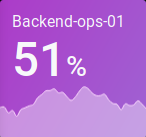
\includegraphics[width=.8\linewidth]{assets/screenshots/Screenshot_2020-12-08 1 - New Features in v7 0 - Grafana.png}
		\captionsetup{justification=centering}
		\caption{Single Metric\\with Graph}
		\label{fig:sfig1}
	\end{subfigure}%
	\begin{subfigure}{.25\textwidth}
		\centering
		
\includegraphics[width=.8\linewidth]{assets/screenshots/Screenshot_2020-12-08 Website trends - Grafana.png}
		\captionsetup{justification=centering}
		\caption{Single Metric\\as Gauge}
		\label{fig:sfig2}
	\end{subfigure}%
	\begin{subfigure}{.5\textwidth}
		\centering
		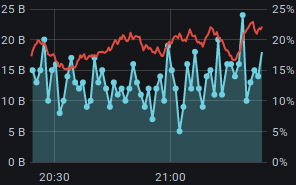
\includegraphics[width=.8\linewidth]{assets/screenshots/Screenshot_2020-12-08 Grafana Play Home - Grafana(2).png}
		\captionsetup{justification=centering}
		\caption{Multimetric plot}
		\label{fig:sfig2}
	\end{subfigure}
	\caption{Beispielhafte Diagrammarten}
	\label{fig:fig}
\end{figure}
Ergänzend gibt es ein simples Tabellenformat, Wabenmuster, Balkendiagramme und viele mehr. Diese sind, wie die Datenquellen, durch Plugins erweiterbar. Dank der Quellcode Offenheit des Projektes können, sofern Bedarf besteht, auch eigene Plugins geschrieben werden.

Um die Diagramme mit Daten aus, in unserem Fall, Prometheus zu befüllen muss in jedem Diagramm eine \gls{promql} Query hinterlegt werden, welche regelmäßig ausgeführt wird. Ein solches Diagramm ist Teil eines sogenannten Panels. Das heißt, ein Panel hat genau ein Diagramm und vice-versa. Diese werden nun in Dashboards zusammengefasst, welche dann eine Übersicht bieten. Hier kann man eine Menge an Panels definieren um diese dann gleichzeitig anzeigen zu lassen.

Es soll noch gesagt sein, dass es höhere Ordnungsstrukturen wie Organisationen gibt oder man Dashboards auch wieder in Playlists und/oder Gruppen zusammen fassen kann. Diese Features werden in dieser Arbeit aber nicht näher betrachtet.

\subsection{Panels}
Da Panels viele Einstellungen haben und damit viele Individualisierungen erlauben werden dieser hier kurz näher erläutert.

Jedes Panel besitzt in erster Linie einen Namen, Beschreibung, Diagrammart, Einstellungen für das Layout und Wertebezug \gls{bzgl} kumulierender Funktionen und verhalten mit null-Werten. In Abhängigkeit zur ausgewählten Diagrammart sind verschiedene Konfigurationen möglich. Achsenbeschriftung, Legende, Grenzwerte für symbolische Kolorierung und andere spezifische Einstellungen.

Alternativ zur durch Keywords möglichen Gruppierung der Metriken ist es durch die Angabe mehrerer \gls{promql} Queries möglich mehrere Metriken in einem Diagramm darzustellen.



